%!TEX root = ./main.tex
\definecolor{vscodeblue}{RGB}{0, 122, 204}
\section{Course Tools: IDE, AI, HTML, GitHub}

\begin{frame}
  \centering
  \Huge
  \textbf{Course Tools: \\IDE, AI, HTML, GitHub, }
\end{frame}


\begin{frame}
  \centering
  \Huge
  \textbf{The Best IDE in the World:}\\
  \textcolor{vscodeblue}{\textbf{Visual Studio Code}} \\[1em]

  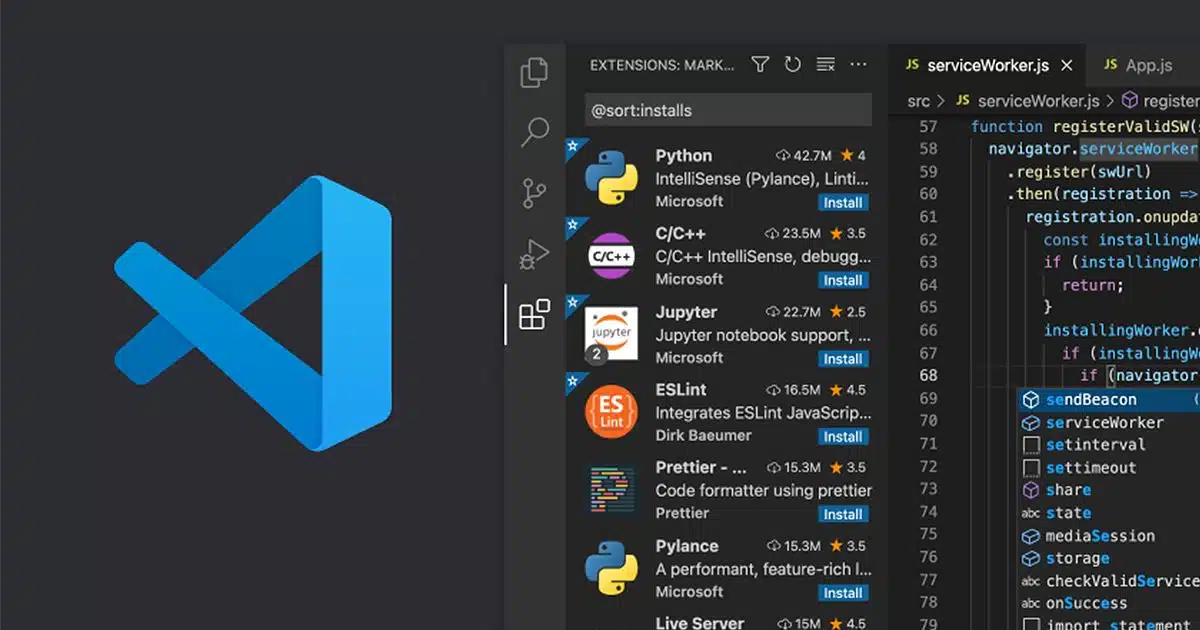
\includegraphics[width=0.92\textwidth]{figure/vs.png}
\end{frame}


\begin{frame}{Become a VS Code Master in 1 Second}
  \LARGE
  \textbf{Just remember one thing:} \\[1em]

  {\centering
  \LARGE
  \textbf{\texttt{Ctrl + Shift + P}} \\[1.5em]
  }

  \large
  This shortcut opens the Command Palette -- your gateway to: \textit{Extensions, settings, themes, terminal, and everything else.}

\end{frame}

\begin{frame}{If Ctrl + Shift + P Is Not Enough}
  \begin{columns}[T]
    \column{0.56\textwidth}
      \centering
      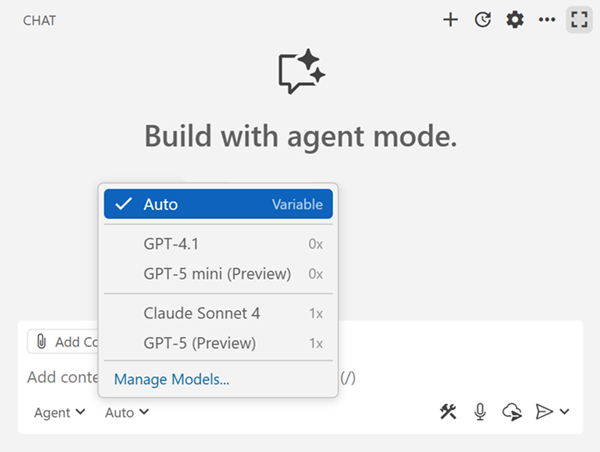
\includegraphics[width=\linewidth]{figure/vscode_agent_models.png}\\[0.35em]
      {\footnotesize VS Code agent mode can work with openAI and Claude models.\par}

    \column{0.44\textwidth}
      \Large
      \textbf{Ask an agent clearly}

      \vspace{0.8em}
      \normalsize
      \begin{itemize}
        \item Give it files, errors, screenshots, and goals
        \item Then verify: compile, run, and read the diff
      \end{itemize}
  \end{columns}
\end{frame}
